
\subsection{Generic Local Search}
\begin{tabular}{m{9cm}m{7cm}}
\begin{enumerate}
    \item An initial solution s
    \item N(s) is the neighborhood of s
    \item L(N(s), s) is the set of legal moves from a solution s
    \item S() selects the move in the legal moves
\end{enumerate}
&
\begin{lstlisting}[mathescape]
Procedure LocalSearch(f,N,L,S,s):
    s* = s
    for k = 1 to MaxTrials do
        if sastifiable(s) $\wedge$ f(s) < f(s*) then
            s* = s
        s = S(L(N (s), s), s)
    return s*
\end{lstlisting}
\end{tabular}

\subsection{Improvement Heuristic}
We can improve this algorithm with two heuristics:
\begin{itemize}
    \item  \textbf{L-Improvement} will only accept moves that improve the solution
    \item \textbf{S-Best} will select one on the move randomely in case of tie.
\end{itemize}

\subsection{Local Minima}

A big problem with local search is that you can be stuck in a local minima(maxima) for a minimization problem(maximimzation).
We have two solutions to get ou of the local minima(maxima) for that:

\begin{tabular}{m{10cm}m{3cm}}
\begin{itemize}
    \item We can accept to \textbf{degrade the solution}.
    \item \textbf{Enlarge the neighborhood}.
\end{itemize}
&
\includegraphics[width=2cm]{localMax}
\end{tabular}

\subsubsection{Degrade the solution}

\paragraph{Constraints types}
\begin{itemize}
    \item \textbf{Hard Constraints} much be respected at all
        time during the local search. (They are enforced at
        initialization)

    \item \textbf{Soft Contstraints} are the constraints that
        can be violated during the search in order to find
        better solutions.
\end{itemize}

For the sudoku example we execute swaps between cases to try to
lower the number of soft constraints violated. Adding more
constraints in the hard constrains makes the initialization
harder but makes the local search process easier.

\paragraph{Tabu meta heuristic}

\begin{itemize}
    \item Whenever you perform a move, this move becomes tabu for a certain
        duration(number of iteration). 
    \item So, when you are stuck in a local minima the
        algorithm keeps iterating between a couple of moves without finding a
        better solution. By making a move tabu you force it to chose some other
        point and escape from the  local minima.

    \item[$\Rightarrow$] If your neightboord is connected and you let the tabu search run
        indefinatly with a long enought tabu periode your algorithm will end up
        finding the optimal solution
\end{itemize}

\paragraph{Improvement on tabu search}
\begin{enumerate}
    \item \textbf{Aspiration}: A move is not considered tabu if it can lead to
        the best so far objective violation.
        So, you not only consider the non tabu moves but you also consider the best
        tabu moves if it improve your best solution and get out of a
        minima.
        
    \item \textbf{Restart}:
        Every X iteration you change randomly some variables in you current
        solution and you restart the from that point. This allows you to travel
        further in the search space in order to maybe find a better solution far
        from the position you were before.
\end{enumerate}


\subsubsection{Enlarge the neighborhood}

\paragraph{Connected Neighborhood}
A neighborhood is connected if and only if for each
solution $s$, there exists a path to an optimal solution $s*$.


This means that if you make the right moves, your neighboord is large
enought to find the optimal solution. However having a connected
neighboord doens't means you will find the optimal solution(in case you
don't make the right moves because of a bad heuristic for
instance).

\begin{itemize}
    \item You don’t necessarily need a restarting strategy (even thought
        this can improve the time to find the best solution)
    \item Randomized heuristics where there is a non zero
        probability of accepting a neighbor$ k \in N(s)$ for each
        solution $s$, may be guaranteed to reach an global
        optimum (example: simulated annealing).
\end{itemize}

\subsection{TSP move}
In order to improve a tour, we can use:

\begin{tabular}{m{3.5cm}m{11cm}}
    \includegraphics[width=4cm]{tsp}
    &
\begin{itemize}
    \item 2-opt which is an algorithm that swap two edges
        to find a better solution.
        \begin{center}
    \includegraphics[width=8cm]{2-opt}
        \end{center}
    \item 3-opt
    \item ...
    \end{itemize}
\end{tabular}
    Note that in practice, the 4-opt is too big to 
    compute.

\subsubsection{Sequential k-opt}

As k-opt is computationally too intensive, we
use \textbf{sequential k-opt}.

\begin{itemize}
    \item A k-Opt move is called sequential if it can be described
        by a path alternating between deleted and added
        edges.
        \begin{center}
    \includegraphics[width=8cm]{6-opt}
        \end{center}

\end{itemize}

The idea is to build greedily a k-Opt move (maybe not the best
move in the k-opt neighboor). At each
step we compute the « gain » of applying it. i.e. the (k
+1)-sequential move is an extension of the k-
sequential move,...

\begin{tabular}{m{10cm}m{6cm}}
$\Rightarrow$ We will start this algorithm with different k's and use the one that gives use to most gain.
&
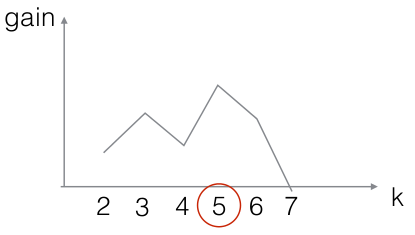
\includegraphics[width=5cm]{linkernighan}
\end{tabular}

\subsubsection{Lin-Kernighan algorithm}
\begin{enumerate}
    \item Let T be the current tour. At each iteration step the
        algorithm attempts to find two sets of edges

        \begin{enumerate}
            \item  We build a set X and Y of edges such that X are the
                deleted edges and Y are the added edges. The edges of X
                are called out-edges and edges of Y are called
                in-edges.

                $\Rightarrow$ If the edges of X are deleted from T and replaced by the
                edges of Y , the result is a better tour.                 
            \item Those edges are
                added elements by elements(empty at start).

        \end{enumerate}
\end{enumerate}

\paragraph{Criteria}

We could start the algorithm just like that but we don't want it to run
forever. This is why we add some \textbf{criteria} to make is sufficiently
efficient.

\begin{itemize}
    %TODO criteria!
    \item \textbf{Sequential exchange criterion}: 
        The sequence $(x1, y1, x2, y2,..., xk, yk)$
        constitutes a chain of adjoining edges.
        $$x_i = (t2i -1, t2i), \quad y_i = (t2i, t2i+1), \quad x_{i+1} =
        (t2i+1, t2i+2)$$

        There must be an added edge followed by a deleted edge.

        \begin{itemize}
            \item[$\Rightarrow$] It's a necessary (but not sufficient) condition that the
        exchange of edges X with edges Y results in a tour is that the
        chain is closed.
    \end{itemize}

    \begin{center}
        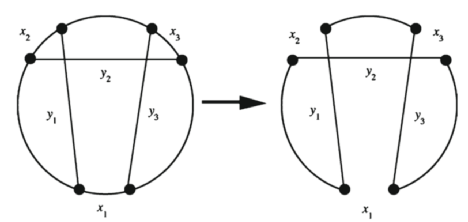
\includegraphics[width=8cm]{seqCriteria}
        \end{center}

\item \textbf{Feasibility criterion}: 
        The resulting configuration must be a cycle.

    \begin{center}
        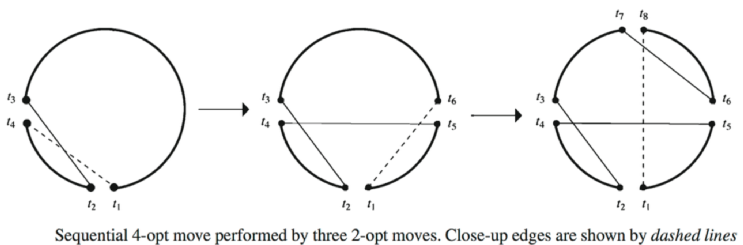
\includegraphics[width=13cm]{feasibleCriteria}
        \end{center}

    \item \textbf{Positive gain criterion}:
        We chose the set Y of edge so that we gain from the nex
        configuration(If the changes gives us a worst solution than the
        one we had before it is not interresting)

    \item \textbf{Disjunctivity criterion}:
        X and Y disjoint(You can't add a deleted edge or you can't
        delete an added edge).

    \item \textbf{Candidate set criterion}:
        When looking for a new edge in Y we limit ourself to only
        considere the 5 nearest neighbors of the vertice.

\end{itemize}

\subsubsection{ATSP reduction to TSP}
Asymetric traveler salesman problem (ATSP)
means that the weight of the edge from A to B isn't necceseraly the
same as the one from B to A. To reduce this problem to the simple TSP we
double every every vertice and put an -inf weight to it.

\begin{center}
    \includegraphics[width=9cm]{ATSP}
\end{center}


\subsection{Vehicle Routing Problem}

\begin{tabular}{m{9cm}m{7cm}}
    This a local search problem mixing the bin packing problem and the TSP problem.
    &
    \includegraphics[width=5cm]{vehicle}
\end{tabular}

We have two types of initializations for this local search:
\begin{itemize}
    \item \textbf{Saving Heuristics}

        \begin{tabular}{m{6cm}m{6cm}}
            \begin{enumerate}
                \item We start with a vehicles \textbf{for each}
                    customer.

                \item Iteratively merge routes to
                    decrease the total distance without exceeding the
                    capacity until no more routes can be
                    merge without violating the capacity constraints.
            \end{enumerate}
            & 
            \includegraphics[width=8cm]{saving}
        \end{tabular}

    \item \textbf{Sweep Heuristic} 

        \begin{tabular}{m{6cm}m{6cm}}
            \begin{enumerate}
                \item  Start with a ray centered at the depot. Turn the
                    ray around the depot and every time we cross a
                    customer with the ray we add it to the current
                    cluster.
                \item If the nest customer exceed the capacity we start a new
                    cluster.
            \end{enumerate}
            & 
            \includegraphics[width=8cm]{sweep}
        \end{tabular}
\end{itemize}

\subsection{Scheduling moves}

\begin{itemize}
    \item Given a set of activities that can not be interrupted and
        that have a certain length and a certain resource need.
    \item A resource with capacity $C$
    \item[$\Rightarrow$] How to minimize the total duration withtou
        exceeding the total capacity.
\end{itemize}

\subsubsection{Iflat-IRelax algorithm (LS)}

We iterativelay flatten then Relax.
\begin{enumerate}
    \item \textbf{Flatten} : We add strong precedences constraints until
        the capacity constrains is satisfied.

        Note that we assume that each
        activity starts as soon as possible while satisfying
        the precedence constraints.

    \item \textbf{Relax} : We remove some precedences randomly on the critical
        path.

        The critical path is that path that is the longest in the
        schedule(the one that makes the schedule the longer).
\end{enumerate}

\subsection{Eternity II}
\begin{itemize}
    \item 16x16 edge matching puzzle
    \end{itemize}

\subsubsection{Swap and rotate}

\begin{enumerate}
    \item Remove $m$ pieces from non edge adjacent positions(up to $n^2/2$ ) 
    \item Replace them optimally:

        \begin{enumerate}
            \item Check score to place them each optimally in holes (by
                check the number of correct adjacent edges)
            \item This generate a complete weighted bipartite graph
                between the removed pieces and holes that we can solve
                thanks to a maximum assignment problem.

                $\Rightarrow$ The size of the Neighborhood is
                exponential but it can be optimally explored in
                polynomial time. (Hungarian algorithm $O(m^3)$)
                \end{enumerate}
\end{enumerate}


\subsection{OscarR CBLS}
\textbf{OscarR CBLS} is a library for local search.
\begin{itemize}
    \item You add the constraints and the objective function and it will
        compute the violations and the delta's for you.
    \item With this you can focus more on the search process(moves and meta-heuristics).
\end{itemize}

\subsection{Exam}
\begin{itemize}
    \item Be able to explain the principle of local search
    \item Be able to implement a simple search with swap-
        moves and a tabu-search meta-heuristic
    \item Be able to suggest a neighborhood for a new problem
        and discuss/prove it it is connected or not.
    \item Be able to explain and apply moves for:
        \begin{itemize}
            \item TSP (Lin-Kernighan) and vehicle routing,
            \item scheduling,
            \item eternity
        \end{itemize}
\end{itemize}
